% !TEX root = ../thesis.tex

\chapter{Experimental Setup}
\label{chap:exp}

\section{Introduction}

\section{The Large Hadron Collider}
\label{sec:LHC}

\section{The Compact Muon Solenoid}
\label{sec:CMS}

\begin{figure}[htbp] % https://cds.cern.ch/record/2665537/
  \centering
  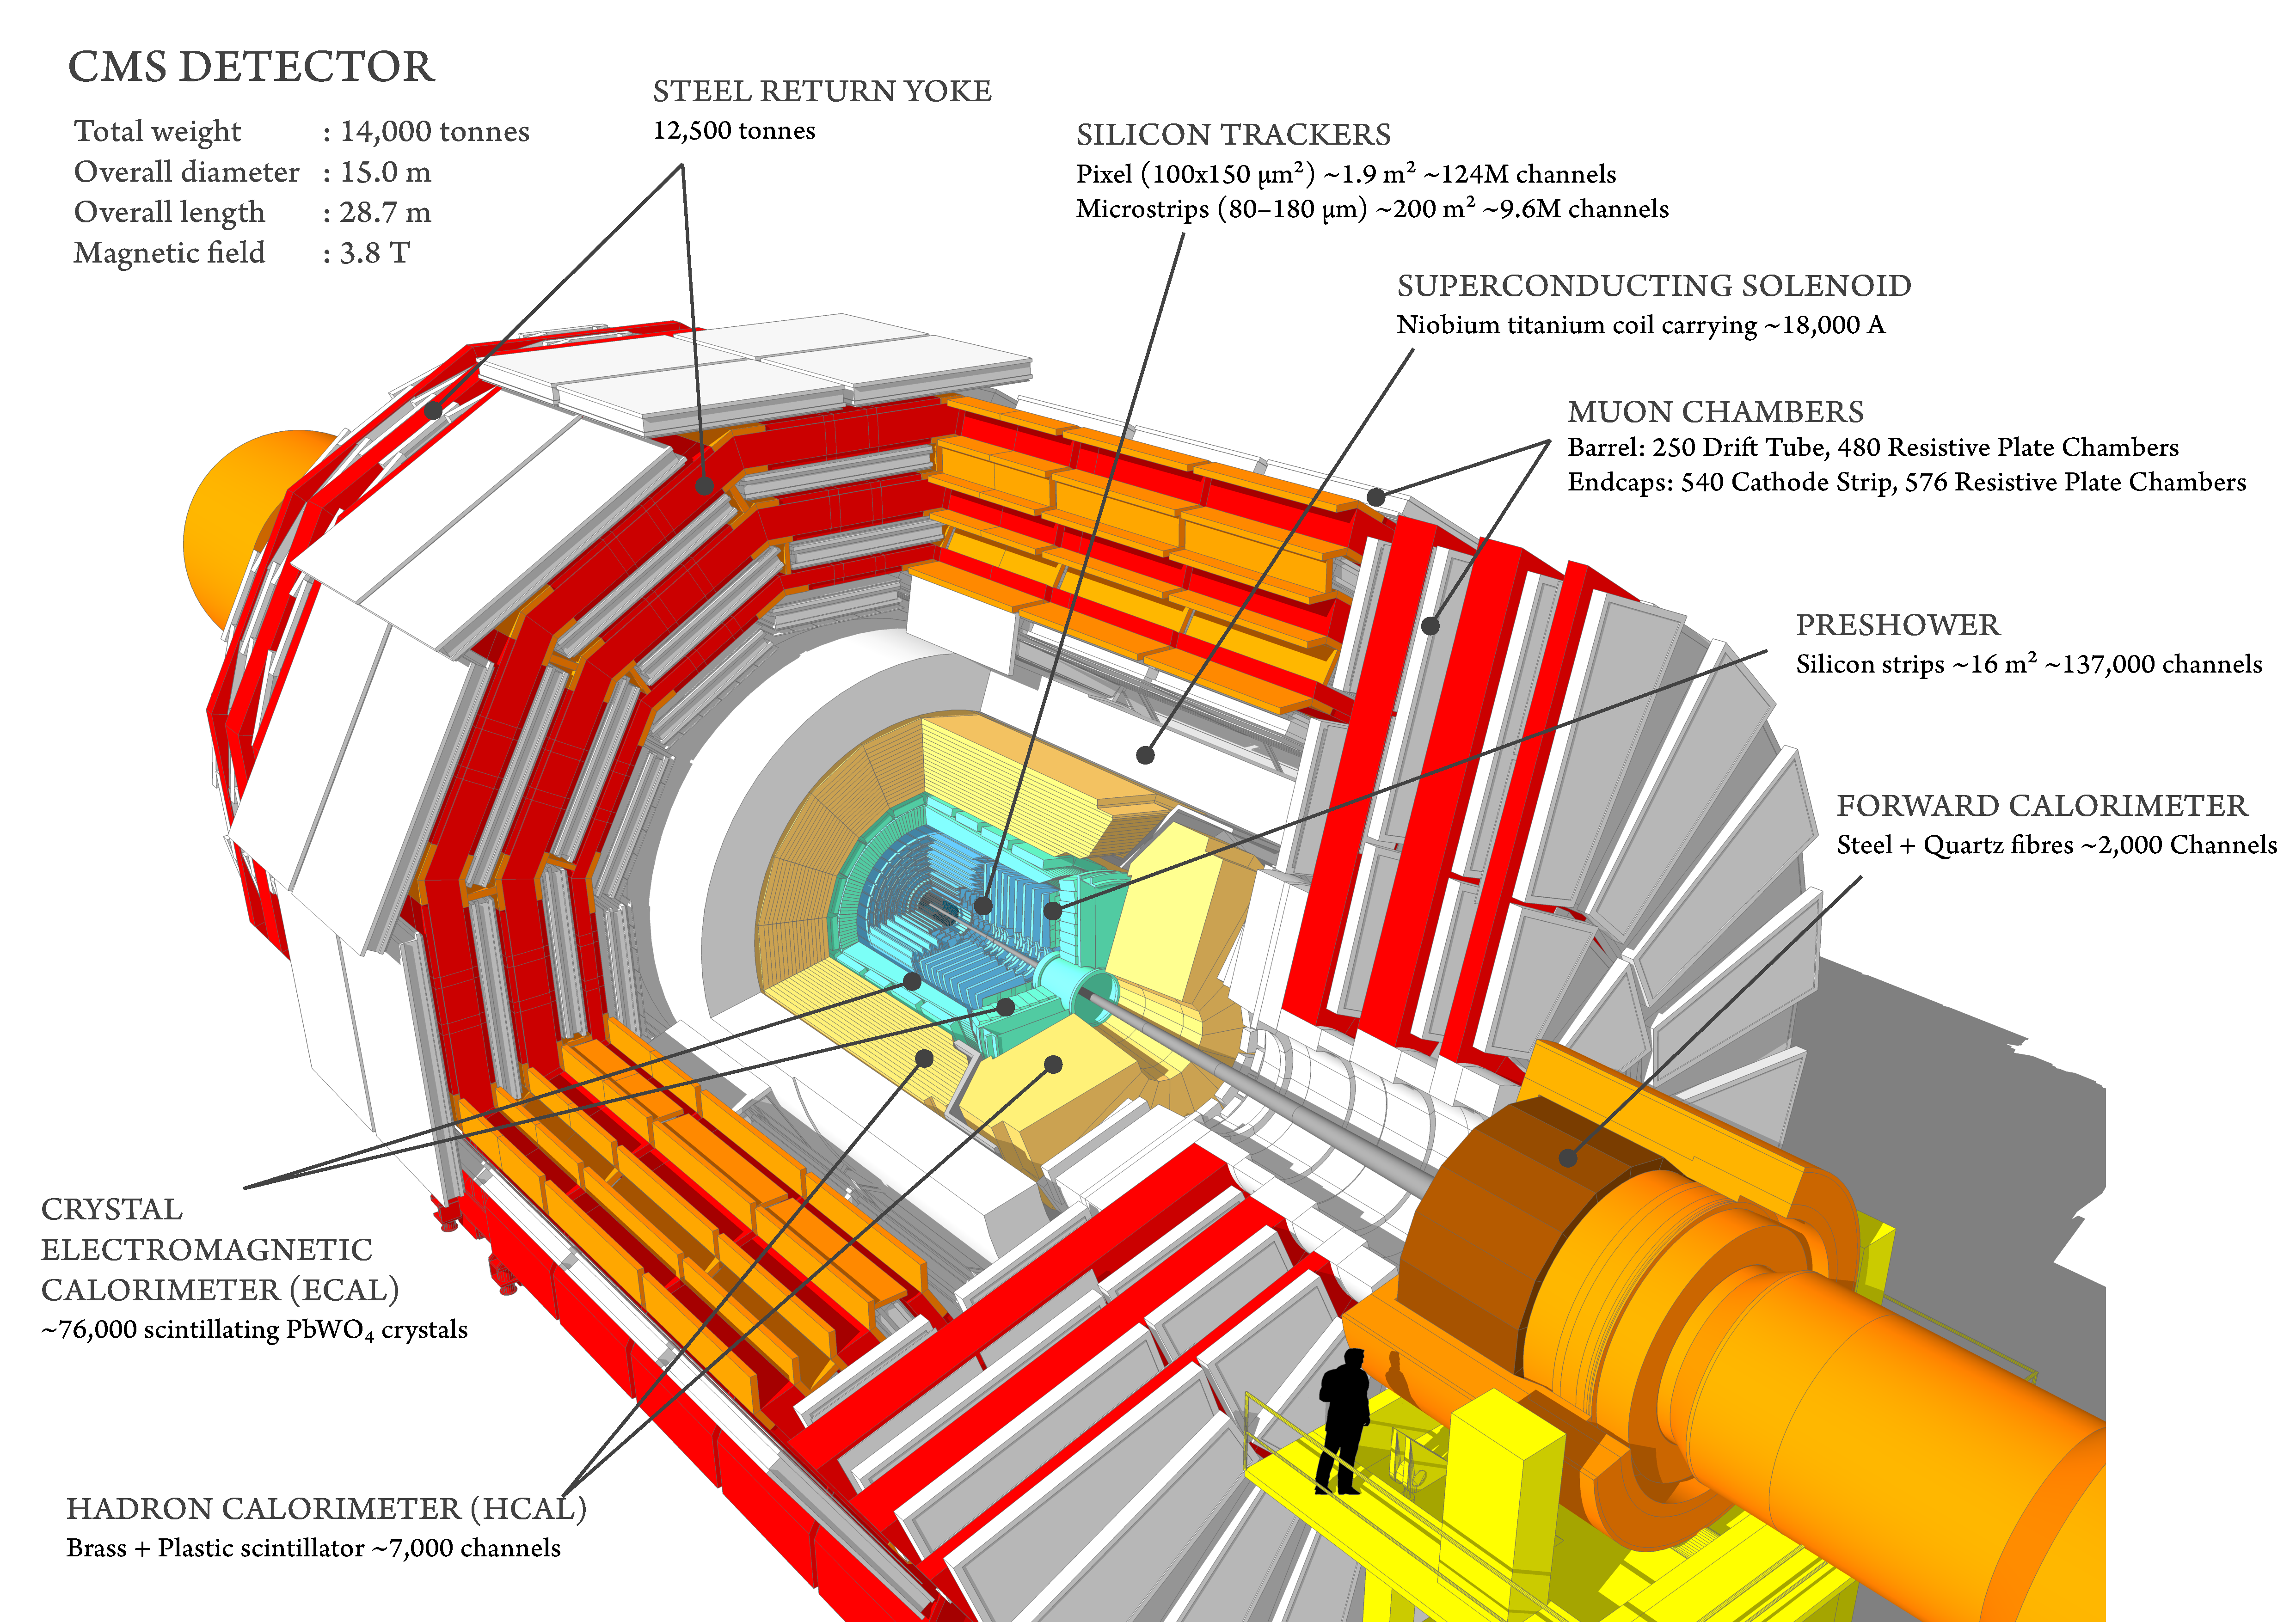
\includegraphics[width=0.85\textwidth]{fig/experiment/cms_cutaway.pdf}
  \caption{}
  \label{fig:CMSCut}
\end{figure}

\begin{figure}[htbp]
  \centering
  \includegraphics[width=0.85\textwidth]{fig/experiment/cms_crosssec.pdf}
  \caption{}
  \label{fig:CMSCrosssec}
\end{figure}

\subsection{Inner Tracking System}
\label{subsec:tracking}

\subsection{Calorimeters}
\label{subsec:calorimeter}

\subsection{Muon Tracking System}
\label{subsec:muonTrack}

\subsection{Trigger System and Data Acquisition}
\label{subsec:trigger}
